\documentclass[a4paper]{article}
\usepackage[UTF8, scheme = plain]{ctex}
\usepackage{graphicx}
\usepackage{epstopdf}
\renewcommand{\baselinestretch}{1.5}


\begin{document}
	\title{\textbf{\begin{flushleft}
				智能棋局:探索人工智能在围棋领域的革新与挑战
	\end{flushleft}}}
	\maketitle
	\author{Aurora, IceCream}
	
	\tableofcontents

	\section{Introduction 介绍}
	\subsection{项目名称}
	本项目名称为"$\Sigma$",选择其为这个项目的标题有三:其一,"$\Sigma$"在数学中有累积与综合的意思;其次,围棋有复杂性与多样性,与"$\Sigma$"相关联;最后,"$\Sigma$"在这里代表策略与概率 , 表示深度学习的策略(Policy)。
	\subsection{实现原理}
	\subsubsection{实现步骤}
	该项目总共需要2个微型控制器同时工作完成,其中一个为MCU,作用为控制四轴机械臂的方向、抓取;另一个识别围棋的位置,预测围棋的落点,并发送到MCU。
	\subsubsection{数据采集}
	通过摄像头选取棋盘各端点,标记出棋盘的位置,通过计算机视觉识别出各格子的情况,绘制出一个复平面,记录各棋子。
	\subsubsection{表示每个棋子的位置}
	在复平面上用向量表示每个棋子\\
	$$ \overrightarrow{z}=(a,b) \Longleftrightarrow z=a+bi $$
	通过二维数组表示这个复平面。
	\subsubsection{训练模型}
	
	
	\section{Goal 目的}
	在人类智慧的璀璨星河中,围棋以其深邃的策略和无穷的变化,被誉为智力游戏的巅峰之作。自古以来,围棋不仅是棋手间智慧的较量,更是文化、哲学乃至人生观的体现。然而,随着科技的发展,特别是人工智能(AI)技术的崛起,这一古老棋艺迎来了前所未有的变革与冲击。
	
	近年来,人工智能在围棋领域的突破性进展,尤其是谷歌DeepMind的\\AlphaGo项目,不仅战胜了世界顶尖的职业棋手,还开启了AI在复杂决策问题上超越人类认知的新纪元。AlphaGo的成功,不仅仅是技术的胜利,更是一次对人类智能边界探索的深刻反思。它证明了深度学习和强化学习算法在解决高度抽象、非线性问题上的强大能力,同时也揭示了AI在未来解决更加复杂社会和科学问题的巨大潜力。
	
	然而,人工智能与围棋的结合并非一帆风顺。AI虽然在计算力和模式识别方面远超人类,但在直觉、情感以及对围棋文化的深层理解上仍存在局限。此外,AI在围棋领域的成功应用,也引发了关于机器智能与人类智能本质差异、人工智能伦理以及未来人机共生关系的广泛讨论。
	
	本论文旨在探讨人工智能在围棋领域的发展历程、关键技术、所面临的挑战以及对未来的影响。我们将分析AlphaGo等AI系统的架构原理,探讨其在围棋决策过程中的创新之处,并评估这些技术在其他领域应用的可行性。同时,我们也将深入讨论AI围棋系统所带来的伦理、文化和教育层面的思考,以期为构建更加和谐的人工智能社会提供有益的视角。
	
	通过本文的研究,我们期望能够加深对人工智能技术及其社会影响的理解,促进人机合作的新模式,同时也为围棋这一古老艺术注入新的活力与思考。
	
	\section{Implementation  实现}
	\subsection{Reinforcement Learning  (深度学习)}
	首先,我们通过C++编写了一个围棋的程序作为深度学习的Environment,再构建出一个Agent(智能体)交互,让Agent自我对弈,且仅在Agent获得整场棋局的胜利后获得Reward(奖励)。在训练足够多轮以后,模型开始收敛,获得胜利的场数比训练前高。\\
	深度学习:
	\begin{figure}[htbp]
		\centering
		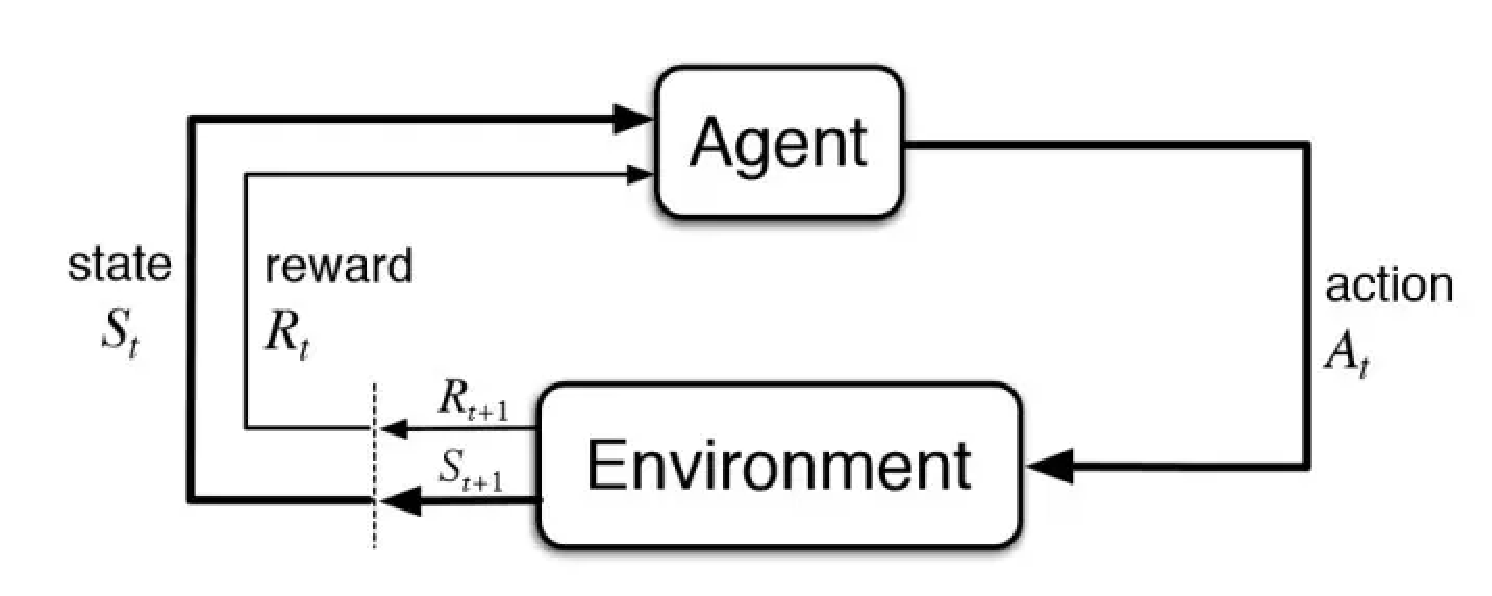
\includegraphics[scale=0.2]{RL.eps}
		\caption{Reinforcement Learning}
		\label{figure}
	\end{figure}\\
	Reward机制是在整场棋局获得胜利后加分,失败时扣分的原因是:若在吃掉对方的棋子时加分,那么Agent会倾向于将对方的棋子吃掉,这对于整场对弈不利,故使用在整场胜利后加分。
	\subsection{主要的实现过程}
	Nothing to show
	
	
	\section{Reflection and prospect 反思与展望}
	Nothing to show
	
	\section{附:训练过程}
	Nothing to show
\end{document}